\chapter{Streaming into the Lakehouse}
\label{ch:streaming}

\begin{chapterintro}
Structured Streaming is the same query engine over an unbounded table, processing
one micro-batch at a time and ending each batch with a single Iceberg commit. The
whole model from the earlier parts still applies --- the shuffle, the executor
budget, the commit --- but with two new pressures: state that must be kept between
batches, and a commit cadence that produces small files faster than a batch job.
This chapter measures both on the lab (\Cref{sec:refenv-lab}): a rate source
writing 20,000 rows per second into an Iceberg table at three trigger intervals,
a windowed aggregation with and without a watermark, the three output modes, a
query killed and restarted from its checkpoint, and \texttt{AvailableNow}
processing a growing directory.
\end{chapterintro}

\section{The micro-batch model and the unbounded table}
\label{sec:stream-microbatch}

Structured Streaming treats a stream as a table that keeps growing, and a
streaming query as an ordinary DataFrame query re-run incrementally against the new
rows since the last run. Each run is a \emph{micro-batch}: the driver's
\texttt{StreamExecution} asks the source for the range of new offsets available,
plans and executes an ordinary batch job over exactly that range --- the same
Catalyst pipeline, the same job/stage/task machinery from \Cref{ch:shape} ---
and, on success, records the offsets it has processed to a \emph{checkpoint}
location before asking for the next range. Nothing about execution is special to
streaming; what is special is that this loop runs forever and that recovery after a
failure means replaying from the last checkpointed offset rather than restarting
the whole computation (\Cref{fig:microbatch-commit-loop}).

\begin{figure}[htbp]
  \centering
  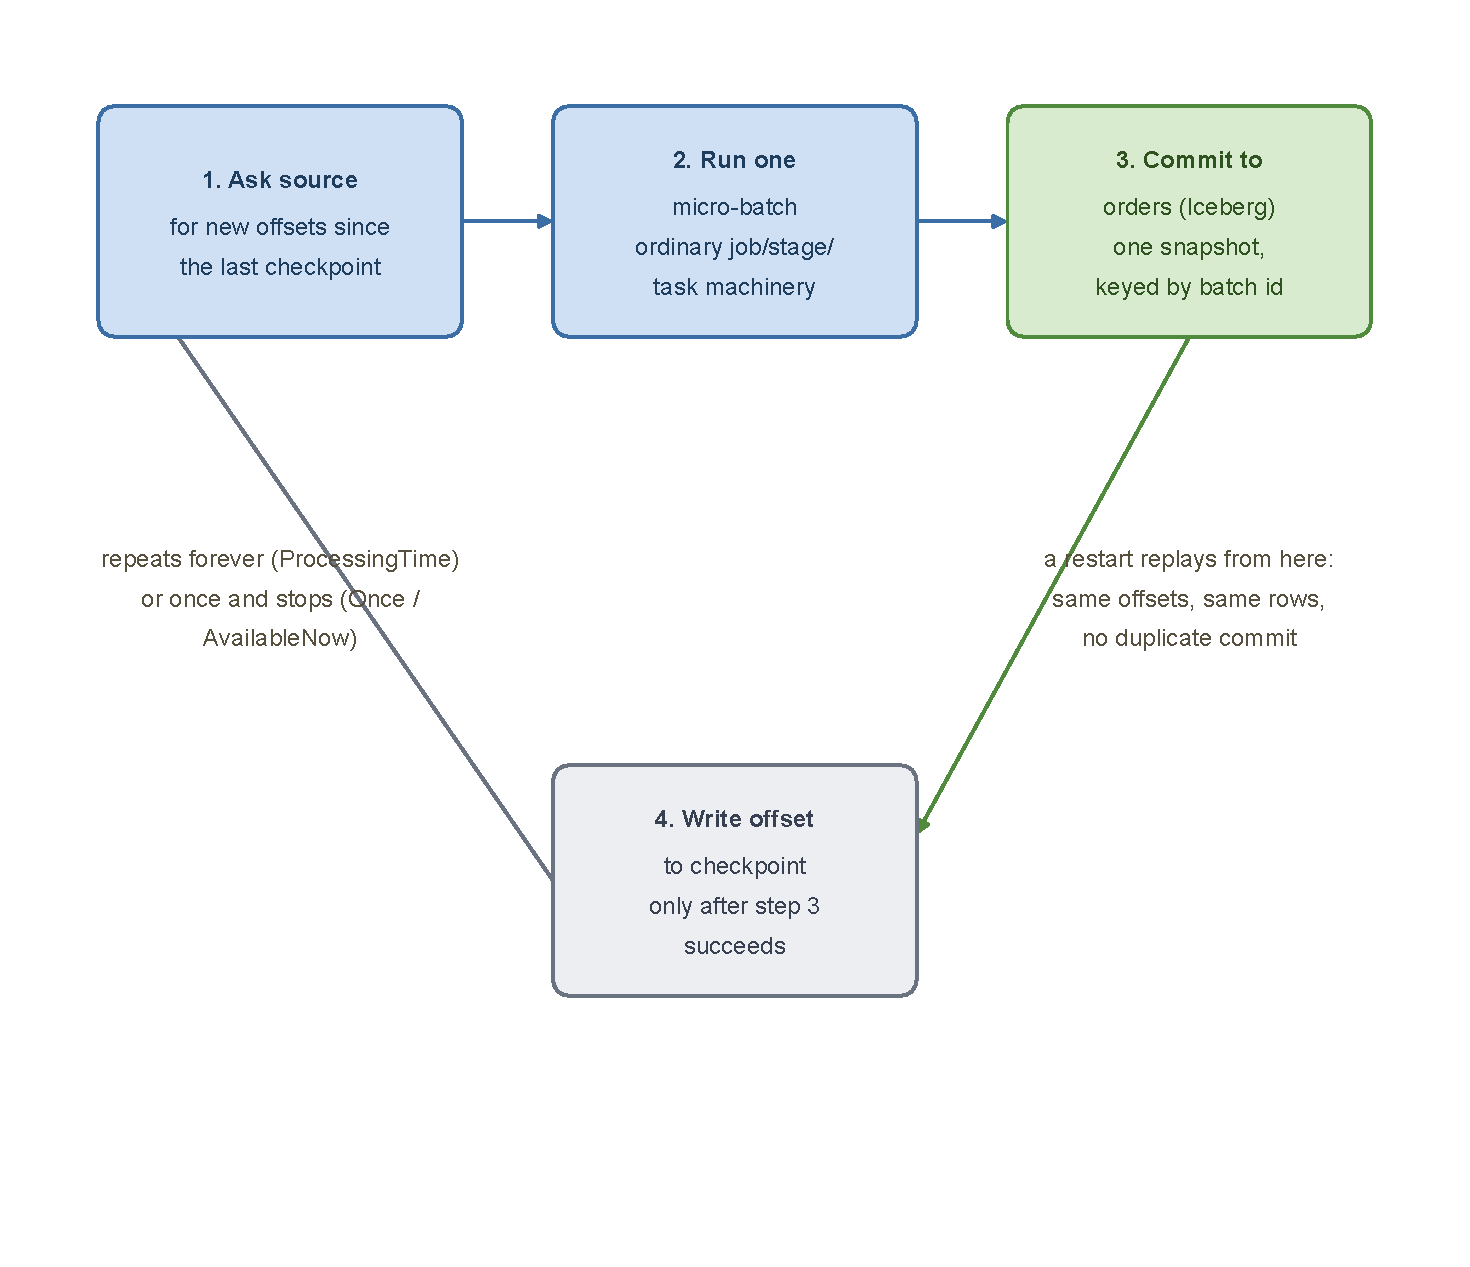
\includegraphics[width=0.85\linewidth]{microbatch-commit-loop.pdf}
  \caption{One iteration of the micro-batch loop. The offset log is written
  before the batch runs and the commit log after it, which is what makes a restart
  safe: a replay re-runs exactly the range that either never committed or already
  did, never anything in between.}
  \label{fig:microbatch-commit-loop}
\end{figure}

The lab's checkpoint directory shows the loop's two logs. After the run described in
\Cref{sec:stream-exactly-once}, the checkpoint held \texttt{offsets/0} through
\texttt{offsets/28} and \texttt{commits/0} through \texttt{commits/28}: one offset
entry and one commit entry per micro-batch, 29 of each, matching the table's 29
snapshots.

\section{Sources and sinks}
\label{sec:stream-sources-sinks}

A source needs one contract: given a starting offset, return the new records since
it, and report the latest offset available. Kafka is the most common source, with a
partition's offset serving directly as the streaming offset; the \texttt{file}
source uses file names as offsets; the lab's \texttt{rate} source generates rows at
a fixed speed and is used here so that the experiments are reproducible. A sink is
symmetric: it must support exactly-once writes idempotently keyed by batch id, or
tolerate the batch being reprocessed. Writing to an Iceberg table satisfies this
because a commit is already atomic (\Cref{sec:ice-commit-swap}): a batch that
failed after writing files but before committing never became visible
(\Cref{fig:dsv2-write-protocol} in \Cref{ch:dsv2} measured that for a batch write).

\section{Event time and watermarking}
\label{sec:stream-watermark}

Grouping by \emph{event time} (when something happened, carried in the data --- the
specimen's \texttt{order\_ts}) rather than \emph{processing time} needs a rule for
when a time-based group is complete, since late data can always arrive for a window
already emitted. A \emph{watermark} (\texttt{withWatermark("order\_ts", "10
minutes")}) declares how late data is tolerated: Spark tracks the maximum
\texttt{order\_ts} seen so far and treats any window ending more than the watermark
delay before that maximum as closed. The rule, applied by hand to one moment of the
stream, looks like this (an arithmetic illustration of the rule, not captured
output):

\begin{lstlisting}[language=text,numbers=none,caption={Which orders close a 10-minute window, and which arrive too late (illustration of the rule)},captionpos=b,label=lst:stream-watermark-rule]
Max order_ts seen so far: 10:47   ->  watermark = 10:37
Window [10:30, 10:40) already closed (ends before 10:37)   -> emitted, forgotten
Window [10:40, 10:50) still open   (ends after 10:37)      -> still accepting rows
An order_ts=10:35 row arrives late -> closed window -> dropped, not counted
An order_ts=10:41 row arrives late -> open window   -> counted normally
\end{lstlisting}

The watermark is also what bounds state. The lab ran the same windowed count
(5-second windows by 1,000 customer keys, 2,000 rows per second) twice for 100
seconds, once without a watermark and once with a 10-second watermark, and
recorded the state store's row count after every micro-batch
(\Cref{fig:state-growth}).

\begin{figure}[htbp]
  \centering
  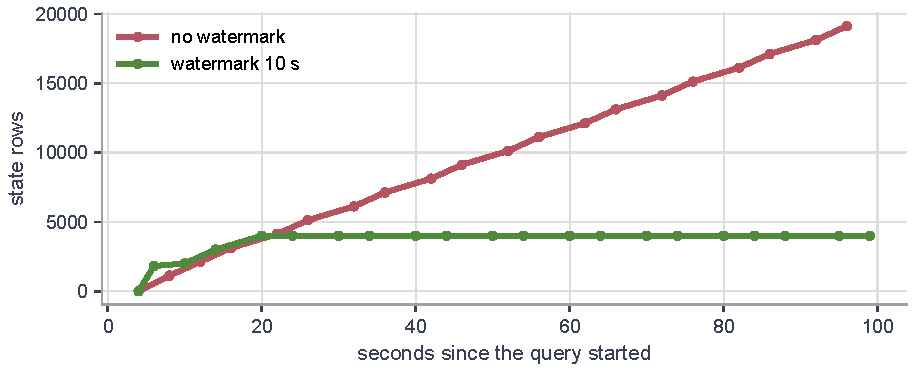
\includegraphics[width=0.9\linewidth]{state-growth.pdf}
  \caption{State rows against time. Without a watermark nothing tells Spark a
  window is complete, so state grows by about 1,000 rows every 5-second window
  and was still climbing (19,121 rows, 5.0~MB) when the run stopped. With a
  10-second watermark it plateaus at 4,000 rows (1.4~MB) as closed windows are
  evicted --- 16,000 rows removed over the run.}
  \label{fig:state-growth}
\end{figure}

A batch aggregate never has this problem: it reads its input once and the state
disappears when the job ends. A streaming aggregation's state keeps accumulating
for as long as the query runs, which is why state size, not input size, is what
eventually threatens the heap in a way no batch operator ever has to plan around.

\section{Stateful operations and the state store}
\label{sec:stream-state}

The \emph{state store} holds the partial results a windowed aggregation or a
streaming join needs across micro-batches, checkpointed alongside the offsets so it
survives a restart. The default provider keeps state as JVM objects in memory per
task and snapshots it to the checkpoint; \texttt{RocksDBStateStoreProvider}
(\conf{spark.sql.streaming.stateStore.providerClass}) moves it into an embedded
RocksDB instance per task --- a log-structured merge tree that never updates a file
in place, flushes a small in-memory buffer as an immutable sorted file, and merges
files in the background. That structure lets it hold more state than fits in the
heap, at the cost of occasional compaction pauses and a disk read for state outside
its block cache.

The lab compared the two providers on a heavier state: 20,000 rows per second into
10-second windows by 40,000 customer keys, 120 seconds, 2~GB heap
(\Cref{fig:state-providers}). At about 520,000 state rows the default provider
reported 144~MB of state memory and the RocksDB provider 22~MB --- 6.5 times less
memory held by the store --- while the micro-batch took 1.2~s against 0.8~s, with
the state-store commit at 1.05~s against 0.53~s. RocksDB trades per-batch latency
for a bounded memory footprint; at this size the lab's heap was not under pressure,
so the benefit shown is footprint, not avoided GC. The two memory figures are not
perfectly comparable --- they are each provider's own accounting.

\begin{figure}[htbp]
  \centering
  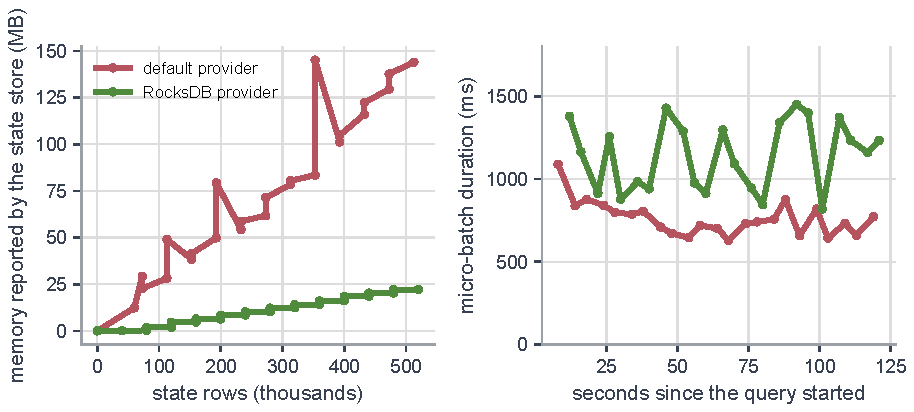
\includegraphics[width=\linewidth]{state-providers.pdf}
  \caption{Left: reported state memory against state rows for the default and RocksDB
  providers. Right: micro-batch duration over time. RocksDB held the same rows in
  one sixth of the reported memory and paid with slower commits.}
  \label{fig:state-providers}
\end{figure}

\section{Output modes and triggers}
\label{sec:stream-modes-triggers}

\emph{Output mode} controls what a micro-batch emits. The lab ran the same
windowed count under all three modes with a 5-second watermark and recorded the
rows each batch emitted (\Cref{fig:output-modes}).

\begin{figure}[htbp]
  \centering
  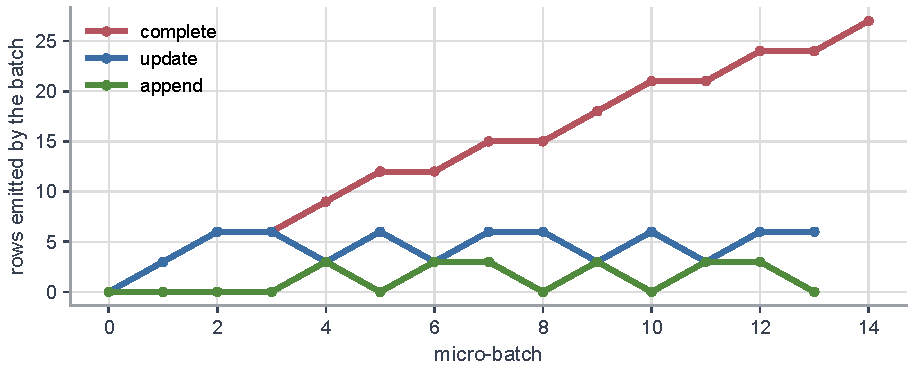
\includegraphics[width=0.9\linewidth]{output-modes.pdf}
  \caption{Rows emitted per micro-batch for the same query. \texttt{append} emits
  nothing until a window closes (0 or 3 rows); \texttt{update} emits the windows
  that changed (3 to 6 rows); \texttt{complete} re-emits the whole result table,
  which grew from 3 to 27 rows over 15 batches and keeps growing.}
  \label{fig:output-modes}
\end{figure}

\texttt{append} is final-only: a row leaves once its window is closed by the
watermark, so output lags the data by the watermark delay. \texttt{update} emits
changes, including rows already emitted before. \texttt{complete} is the one that
does not scale: its output is every window ever seen, so its cost grows with the
life of the query --- viable only for a small, bounded aggregate.

\emph{Trigger} controls when a micro-batch runs. \texttt{ProcessingTime} fires on
a fixed interval; \texttt{AvailableNow} reuses the same loop for one iteration over
everything available and exits, which turns a streaming query into a scheduled
incremental job. The lab ran it three times against a directory of Parquet files
(\Cref{tab:stream-availnow}).

\begin{table}[htbp]
\centering\footnotesize
\renewcommand{\arraystretch}{1.2}
\begin{tabular}{@{}rrrrr@{}}
\toprule
\textbf{Run} & \textbf{New rows landed} & \textbf{Seconds} & \textbf{Table rows} & \textbf{Snapshots} \\
\midrule
1 & 100,000 & 6.6 & 100,000 & 1 \\
2 & 0 & 1.6 & 100,000 & 1 \\
3 & 50,000 & 4.2 & 150,000 & 2 \\
\bottomrule
\end{tabular}
\caption{\texttt{Trigger.AvailableNow} over a directory that grows between runs.
The first run processes everything, the second finds nothing and commits nothing
(no empty snapshot), and the third processes only the new files.}
\label{tab:stream-availnow}
\end{table}

\section{Exactly-once and the commit}
\label{sec:stream-exactly-once}

``Exactly-once'' is two guarantees, neither sufficient alone: the checkpoint's
offset log records which input range a batch covers before the batch runs, so a
restart replays the same range rather than skipping or duplicating input; and the
sink makes committing that range idempotent. For Iceberg the sink writes its
identity into each snapshot's summary. The lab read it back from a streaming-written
table:

\begin{lstlisting}[language=text,style=plan,caption={Streaming identity recorded in a snapshot summary (Iceberg 1.6.1, selected keys)},captionpos=b,label=lst:stream-summary]
spark.sql.streaming.queryId   = c3fa69d9-60d4-4f1b-b5a2-a55d422fe0f3
spark.sql.streaming.epochId   = 49
added-data-files = 1     added-records = 40000     added-files-size = 65127
\end{lstlisting}

The keys are \conf{spark.sql.streaming.queryId} and
\conf{spark.sql.streaming.epochId}: the query that wrote the snapshot and the
micro-batch number. The lab tested the replay directly: after a query had committed epochs 0 to 8, the
last commit-log entry (and its checksum file) was deleted, which makes Spark believe
epoch 8 never committed, and the query was restarted. It re-ran epoch 8, carried on to
epoch 23, and the table held 79,000 rows, all distinct, with epoch 8 appearing in
exactly one snapshot. A replayed batch that had already committed was not committed
twice.

The lab then tested the behaviour end to end. A query writing 2,000 rows per second
into a fresh table with a 3-second trigger was killed with \texttt{docker kill}
about 60 seconds in, and restarted with the same checkpoint for another 30 seconds.
The result (\Cref{fig:kill-restart}):

\begin{figure}[htbp]
  \centering
  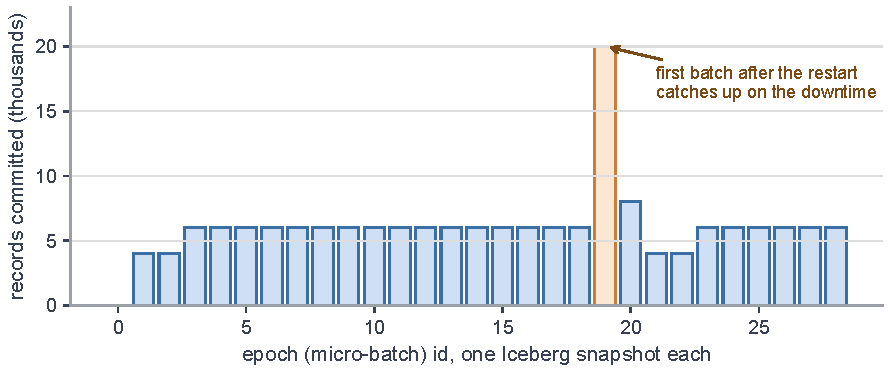
\includegraphics[width=0.9\linewidth]{kill-restart.pdf}
  \caption{Records per snapshot across a kill and restart. The table ended with 29
  snapshots whose epoch ids run 0 to 28 without a gap under one query id; the
  first batch after the restart (epoch 19) carried 20,000 records, catching up on
  the downtime. The table held 176,000 rows, all distinct, covering sequence
  numbers 0 to 175,999 with no gap.}
  \label{fig:kill-restart}
\end{figure}

No row was duplicated or lost, and the 28 data files on disk equalled the 28 in the
table, so the kill left no orphan. The experiment does not prove that a kill in the
narrow window between writing files and committing is safe --- it cannot say where
in the batch the kill landed --- but it shows the replay behaviour on a real kill:
the restart resumed from the checkpoint's last batch and the offset range it
covered.

\section{Writing to Iceberg: cadence, small files, maintenance}
\label{sec:stream-iceberg-write}

Every micro-batch that writes to Iceberg ends in exactly one commit --- one new
snapshot, one new manifest list, at least one new manifest --- regardless of how
little data it contained. The lab ran the same 20,000-rows-per-second stream into
a day-partitioned table at three trigger intervals for 100 seconds each
(\Cref{fig:stream-cadence}).

\begin{figure}[htbp]
  \centering
  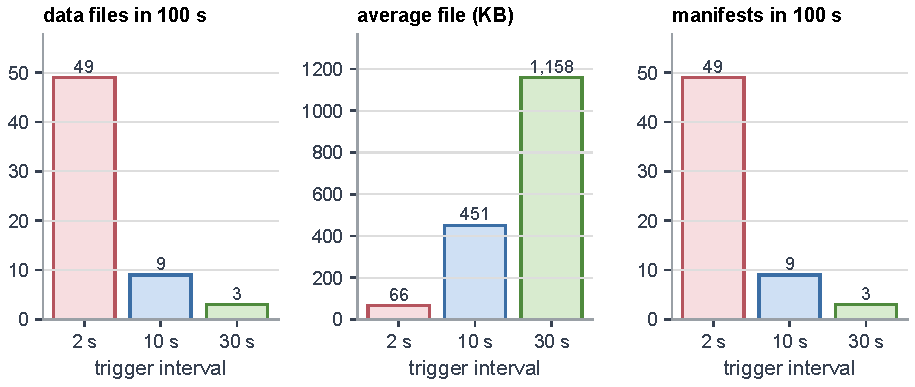
\includegraphics[width=\linewidth]{stream-cadence.pdf}
  \caption{The trigger interval sets the commit count, and with it the file count,
  the file size and the manifest count. A 2-second trigger produced 49 files of
  66~KB and 49 manifests in 100 seconds; a 30-second trigger produced 3 files of
  1.16~MB and 3 manifests.}
  \label{fig:stream-cadence}
\end{figure}

\begin{table}[htbp]
\centering\footnotesize
\renewcommand{\arraystretch}{1.2}
\begin{tabular}{@{}rrrrr@{}}
\toprule
\textbf{Trigger} & \textbf{Snapshots / 100 s} & \textbf{Files / 100 s} & \textbf{Average file} & \textbf{Files per day (extrapolated)} \\
\midrule
2 s & 50 & 49 & 66 KB & about 42,000 \\
10 s & 10 & 9 & 451 KB & about 7,800 \\
30 s & 4 & 3 & 1,159 KB & about 2,600 \\
\bottomrule
\end{tabular}
\caption{The lab's measurements and their extrapolation to a day
($\times 864$). Each trigger produced one file per commit because the table has one
partition for the day; the lab's rate (about 1.7 bytes per row after compression)
is far lower than a production stream, so the shape of the relationship is the
transferable part, not the absolute sizes.}
\label{tab:stream-cadence}
\end{table}

The relationship is exact and simple: files, snapshots and manifests grow as one
over the trigger interval, and average file size grows in proportion to it. A
stream with a short trigger is therefore the fastest way to produce the
small-files and manifest-growth problems of \Cref{ch:iceberg-write}. The lever is
the trigger interval against the latency budget --- decide the interval from how
fresh a row must be, then treat continuous compaction
(\Cref{sec:ice-write-compaction}) as the backstop for the file size that interval
implies, not as a substitute for choosing it.

\section{From symptom to lever}
\label{sec:stream-levers}

\begin{table}[htbp]
\centering\footnotesize
\renewcommand{\arraystretch}{1.25}
\begin{tabular}{@{}p{3.1cm}p{3.7cm}p{4.1cm}p{3.2cm}@{}}
\toprule
\textbf{Symptom} & \textbf{Evidence} & \textbf{Lever} & \textbf{Cost} \\
\midrule
thousands of tiny files per day & \texttt{files}: 66~KB average at a 2~s trigger & widen the trigger; compact continuously & latency; a rewrite job \\
manifests multiply with commits & \texttt{manifests}: one per commit (49 in 100~s) & \texttt{rewrite\_manifests} on a schedule & a metadata rewrite \\
state grows without bound & state rows still rising at the end of the run & add a watermark (4,000-row plateau) & late rows dropped \\
output table grows every batch & \texttt{complete} mode: 3 to 27 rows in 15 batches & use \texttt{update} or \texttt{append} & none \\
need a scheduled job, not a service & \texttt{AvailableNow}: a no-data run commits nothing & \texttt{AvailableNow} from a cron job & start-up time per run \\
duplicate or missing rows after a crash & row count vs distinct count; epoch ids with a gap & same checkpoint, same query id & none \\
\bottomrule
\end{tabular}
\caption{The streaming levers: symptom, evidence, lever, cost.}
\label{tab:stream-levers}
\end{table}

\section{Summary}
\label{sec:stream-summary}

A streaming query is an ordinary batch query re-run incrementally over new offsets,
recovering by replaying from a checkpoint; the lab's checkpoint held one offset and
one commit entry per micro-batch. A watermark is what makes a windowed aggregation
ever finish a window and what bounds state: without it state grew without limit
(19,121 rows and counting), with it state plateaued at 4,000. Output mode decides
what a batch emits, and \texttt{complete} re-emits a result that grows for the life
of the query. Exactly-once combines the offset log with an idempotent sink; Iceberg
records \texttt{queryId} and \texttt{epochId} in each snapshot, and a killed and
restarted query produced 176,000 distinct rows with no gap and no orphan file.
Every commit's fixed overhead multiplied by a short trigger is the cause of a
streaming table's small-files and manifest pressure: 49 files in 100 seconds at a
2-second trigger against 3 at 30 seconds.

\exercisehead
\begin{exercises}
\item Given a trigger interval and an input rate, estimate files committed per
      hour and the compaction cadence needed to keep the table healthy.
\item Run a windowed aggregation with and without a watermark; read
      \texttt{stateOperators.numRowsTotal} from \texttt{recentProgress} after each
      batch and plot it.
\item Kill a streaming query mid-batch and restart it with the same checkpoint.
      Confirm from the table's snapshot summaries that the epoch ids have no gap
      and that the row count equals the distinct count of a unique column.
\end{exercises}
